A dataset of 2747 images was scraped from public Instagram posts from
hashtags by using Puppeteer \footnote{\url{https://pptr.dev/}} (A javascript web-scraper). The dataset
consists of 5 classes, beach, clubbing, nature, drinks, football with
the potential to add more classes in the future. If a person’s image
post falls under a certain category, more activities leaning towards
that activity will be suggested in the itinerary and therefore a
person’s preferences are collected automatically from Instagram posts
and stories. The Beach dataset contains images of seaside, swimming
and summer related activities, the Nature dataset contains images
related to greenery and landscapes, the clubbing dataset contains
crowds and people dancing in a club, the drinks dataset contains
images of cocktails and people in a bar and the football dataset
contains images of stadiums for sport fans. 

    \begin{figure}[H]
        \caption{The image shows a sample image form each of the category}
        \centering
        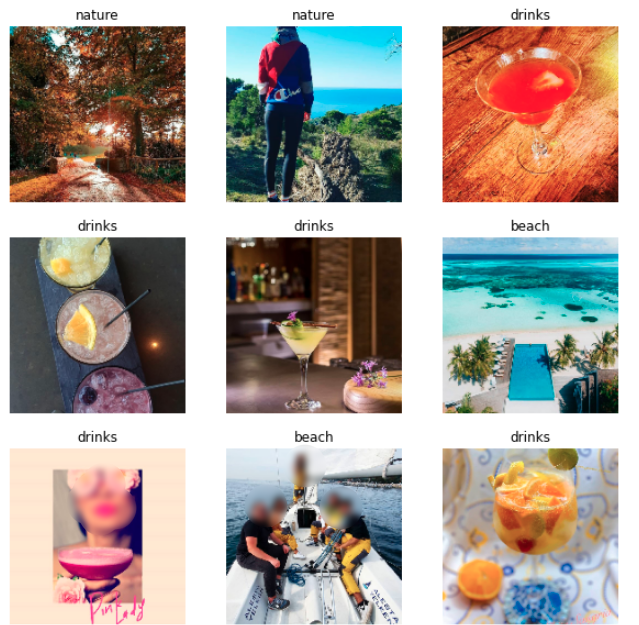
\includegraphics[scale=0.3]{dataset.png}
        \label{dataset}
    \end{figure}
